
\section{Effet Doppler}
\label{effet-doppler}

\subsection{Mise en situation}

\begin{figure}
\centering
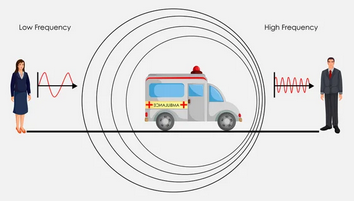
\includegraphics[width=8.557cm,height=4.856cm]{Pictures/1000000100000162000000C9EFEF725F14698266.png}
\caption{}
\end{figure}

Lorsqu'une source d'ondes sonores se déplace, on observe que la
fréquence du son entendu est différente du son qu'on entendrait si la
source est immobile.

Par exemple, lorsque la sirène d'une ambulance ou d'une voiture de
police s'approche d'un auditeur, le son perçu par l'auditeur est plus
aigu (fréquence plus élevée).

Lorsque la sirène d'une ambulance ou d'une voiture de police s'éloigne
d'un auditeur, le son perçu par l'auditeur est plus grave (fréquence
plus basse).

Il y a également un changement de fréquence si l'observateur est en
mouvement et la source est immobile. Le son est plus aigu quand on se
dirige vers la source et plus grave quand on s'éloigne de la source.

Ce changement de fréquence du au mouvement de l'observateur ou de la
source porte le nom d'effet Doppler puisque la théorie décrivant cet
effet fut développée par le physicien allemand Christian Doppler en
1842.

\subsection{Étude quantitative}

Trois situations peuvent être traitées~:
\begin{enumerate}
	\item L'observateur s'éloigne ou se rapproche de la source fixe.
	\item La source s'éloigne ou se rapproche d'un observateur fixe.
	\item La source et l'observateur bougent successivement l'un par rapport à l'autre.
\end{enumerate}

Nous supposerons pour chacune des situations que l'observateur ou la
source se déplace suivant une trajectoire rectiligne et à vitesse
constante.

La différence de fréquence entre celle émise et celle perçue est due à
une variation de la longueur d'onde perçue par l'observateur.

\begin{figure}
\centering
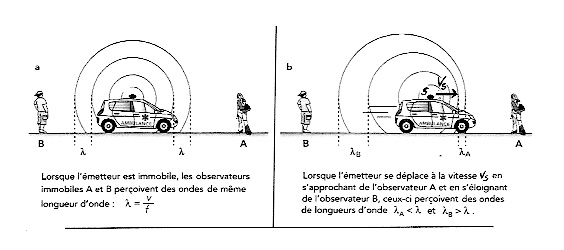
\includegraphics[width=16.611cm,height=7.362cm]{Pictures/1000000100000234000000FA4BFBBF5E6B58FB9F.png}
\caption{}
\end{figure}

\subsection{Une source en mouvement s'approche de l'observateur fixe à une vitesse $v_s$}

Nous noterons~:
\begin{enumerate}
	\item $v_s$~: la vitesse de la source
	\item $v$~: la vitesse de l'onde.
	\item $f$~: la fréquence émise par la source
\end{enumerate}

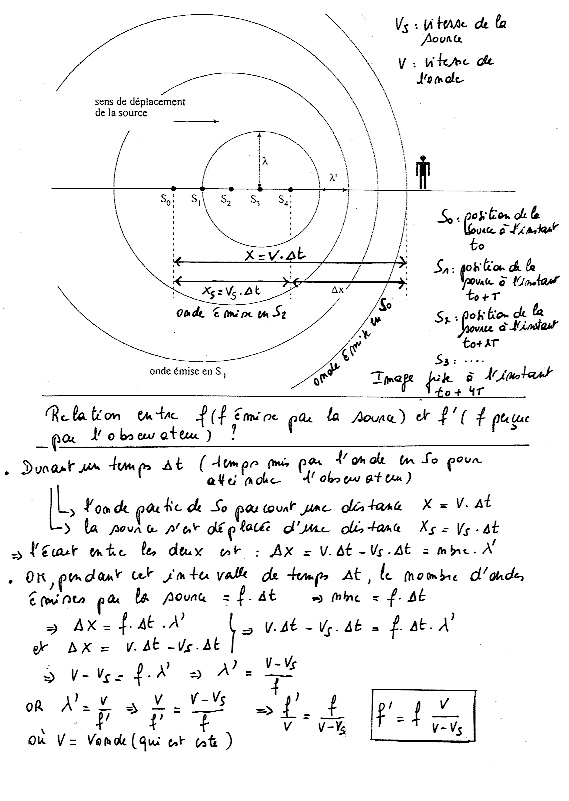
\includegraphics[width=17.231cm,height=24.262cm]{Pictures/10000001000002390000032125422D51A14758E6.png}\textbf{f
`~: la fréquence perçue par l'observateur. }

Nous pourrions dans le même état d'esprit, démontrer les relations entre
$f$ et $f'$ pour les autres situations~:
\begin{enumerate}
	\item L'observateur s'éloigne ou se rapproche de la source fixe.
	\item La source s'éloigne d'un observateur fixe.
\end{enumerate}

Je vous laisse le plaisir de les réaliser.

En résumé, voici les relations pour les 4 situations~:
\begin{figure}
\centering
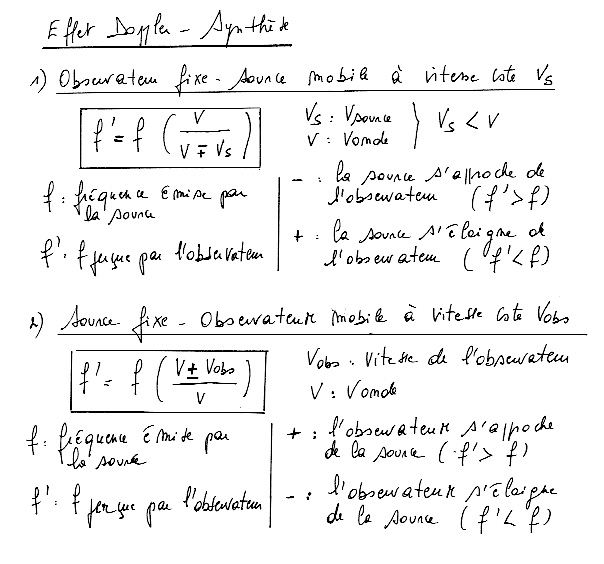
\includegraphics[width=17.866cm,height=17.32cm]{Pictures/100000010000025C00000234BE3EA55298C88B1D.png}
\caption{}
\end{figure}

\subsection{Exercices}

\subsubsection{Exercice 1}% (N°14 du livre p 79)

La fréquence d'une sirène est de 600 Hz (perception au repos).

Si un observateur perçoit ces ondes avec une fréquence de 580 Hz, y
a-t-il éloignement ou rapprochement entre lui et la sirène~?

\subsubsection{Exercice 2} %(N°18 du livre p 80)

La sirène d'une voiture de police a une fréquence de 1200 Hz. Quelle est
la fréquence entendue par un observateur immobile si la voiture se
déplace à 108 km/h~:
\begin{enumerate}
	\item vers l'observateur~?
	\item en s'éloignant de l'observateur~?
\end{enumerate}

\subsubsection{Exercice 3} %(N°19 du livre p 80)

Une source sonore émet à une fréquence de 600 Hz. Ce signal est perçu par
un observateur immobile avec une fréquence de 640 Hz lorsque la source
s'approche de lui. Calculer la fréquence perçue si la source s'éloigne à
la même vitesse.

\subsubsection{Exercice 4} % (N°20 du livre p 80)

La sirène d'une voiture de police a une fréquence de 600 Hz. La voiture
s'approche d'un grand mur à la vitesse de 108 km/h. Calculer la
fréquence du son réfléchi entendu par le policier dans la voiture.

\subsubsection{Exercice 5} % (N°21 du livre p 80)

Debout sur le trottoir, un piéton perçoit une fréquence de 510 Hz
provenant de la sirène d'une voiture de police qui s'approche. Après le
passage de la voiture, la fréquence perçue du son de la sirène par le
piéton est de 430Hz. Calculer la vitesse de la voiture.

\subsubsection{Exercice 6 }

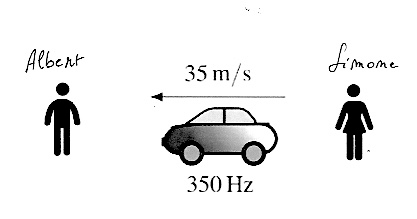
\includegraphics[width=7.4cm,height=3.882cm]{Pictures/10000001000001A1000000DB0C45621DF12277A1.png}
Simone, conducteur d'une auto, fait fonctionner son klaxon, qui a une fréquence de
350 Hz, pour prévenir Albert qui est distrait sur la rue.
\begin{enumerate}
	\item Quelle est la fréquence du son entendu par Albert?
	\item Quelle est la longueur d'onde du son perçu par Albert?
	\item Quelle est la fréquence du son entendu par Simone~?
	\item Quelle est la longueur d'onde du son perçu par Simone~?
\end{enumerate}

(Rép~: 390 Hz~; 87 cm~; 317 Hz~; 1,07 m)

\subsubsection{Exercice 7}

La raie spectrale de l'hydrogène ayant normalement une longueur d'onde
de 656,279 nm a une longueur d'onde de 656,263 nm dans le spectre de
l'étoile Sirius observé sur la Terre. À quelle vitesse Sirius
s'approche-t-elle ou s'éloigne-t-elle de nous?

(Rép~:7314 m/s)
